\documentclass[11pt]{article}
\usepackage[textwidth=18.0cm, textheight=23.0cm, top=2.0cm]{geometry}
\usepackage{pst-all}
\usepackage{amssymb}
\usepackage{tikz}
\usepackage{underscore}\begin{document}
\pagestyle{empty}


ClassName: \underline{\textbf{Class_02.2bp-0}}
\par
BinSize: \underline{\textbf{30 × 30}}
\par
ReduceSize: \underline{\textbf{30 × 30}}
\par
TypeNum: \underline{\textbf{18}}
\par
Num: \underline{\textbf{20}}
\par
OutS: \underline{\textbf{900}}
\par
InS: \underline{\textbf{648}}
\par
Rate: \underline{\textbf{0.720}}
\par
UB: \underline{\textbf{1}}
\par
LB0: \underline{\textbf{1}}
\par
LB: \underline{\textbf{1}}
\par
LBWithCut: \underline{\textbf{1}}
\par
NodeCut: \underline{\textbf{0}}
\par
ExtendedNodeCnt: \underline{\textbf{1}}
\par
GenNodeCnt: \underline{\textbf{1}}
\par
PrimalNode: \underline{\textbf{0}}
\par
ColumnCount: \underline{\textbf{1}}
\par
TotalCutCount: \underline{\textbf{0}}
\par
RootCutCount: \underline{\textbf{0}}
\par
LPSolverCnt: \underline{\textbf{1}}
\par
PricingSolverCnt: \underline{\textbf{0}}
\par
BranchAndBoundNum: \underline{\textbf{1}}
\par
isOpt: \underline{\textbf{true}}
\par
TimeOnInitSolution: \underline{\textbf{600.000 s}}
\par
TimeOnPrimal: \underline{\textbf{0.000 s}}
\par
TimeOnPricing: \underline{\textbf{0.000 s}}
\par
TimeOnRmp: \underline{\textbf{0.078 s}}
\par
TotalTime: \underline{\textbf{600.313 s}}
\par
\newpage


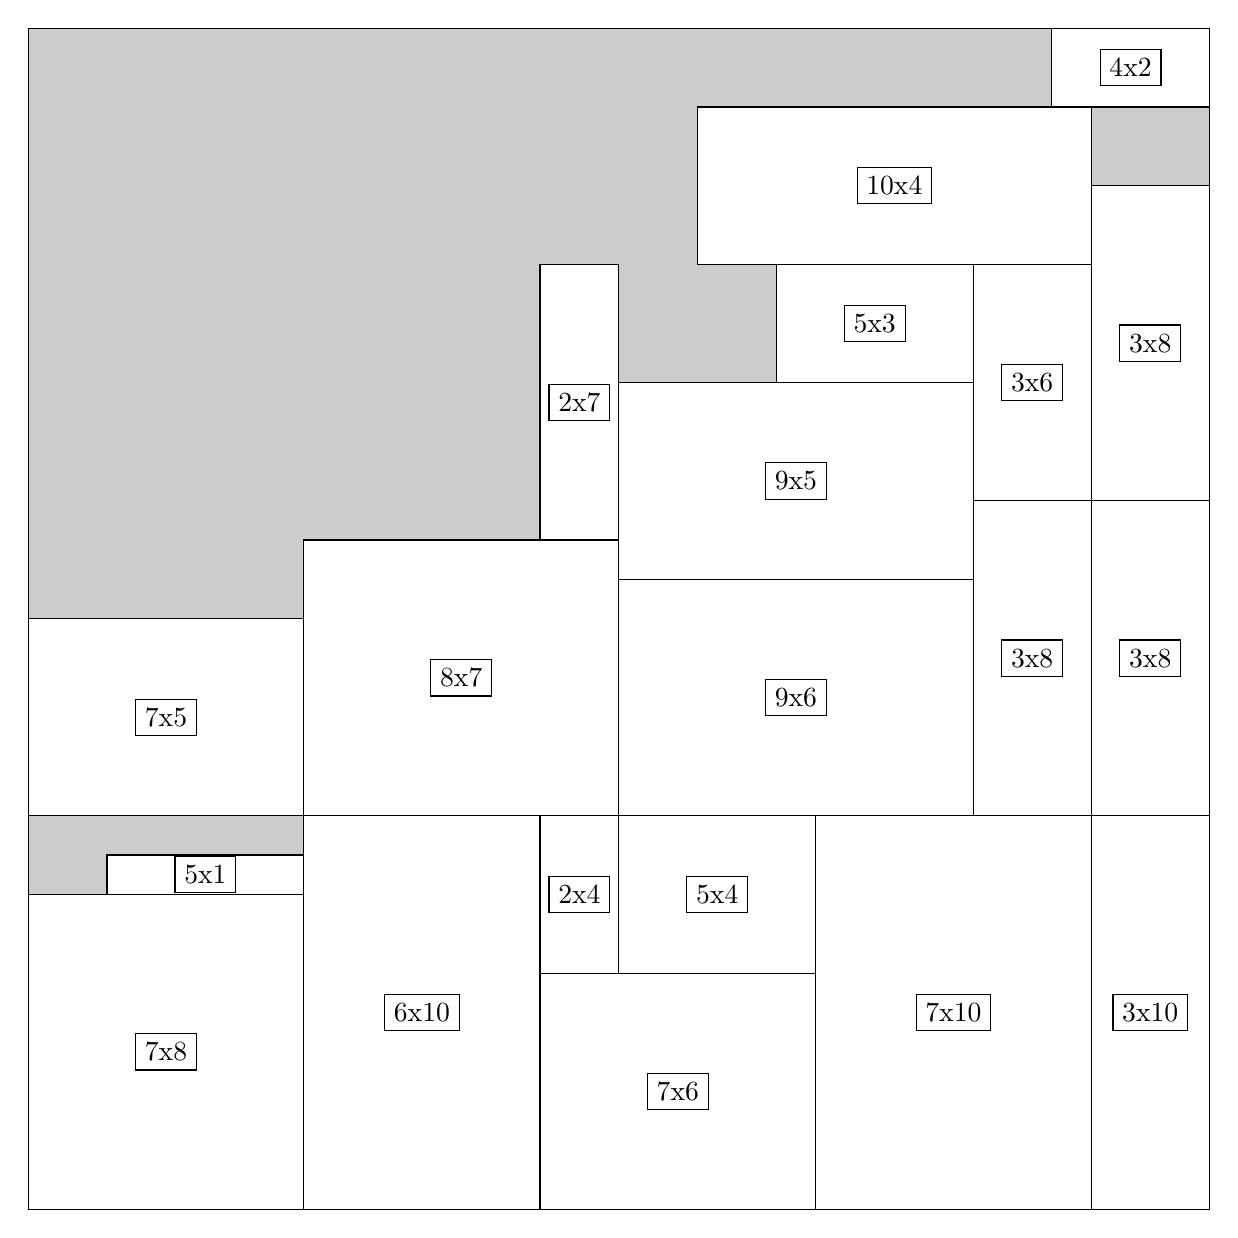
\begin{tikzpicture}[shorten >=1pt,scale=1.0,every node/.style={scale=1.0},->]
\tikzstyle{vertex}=[circle,fill=black!25,minimum size=14pt,inner sep=0pt]
\filldraw[fill=gray!40!white, draw=black] (0,0) rectangle (15.0,15.0);
\foreach \name/\x/\y/\w/\h in {3x10/13.5/0.0/1.5/5.0,3x8/13.5/5.0/1.5/4.0,3x8/13.5/9.0/1.5/4.0,7x10/10.0/0.0/3.5/5.0,7x6/6.5/0.0/3.5/3.0,5x4/7.5/3.0/2.5/2.0,2x4/6.5/3.0/1.0/2.0,6x10/3.5/0.0/3.0/5.0,7x8/0.0/0.0/3.5/4.0,5x1/1.0/4.0/2.5/0.5,3x8/12.0/5.0/1.5/4.0,3x6/12.0/9.0/1.5/3.0,9x6/7.5/5.0/4.5/3.0,9x5/7.5/8.0/4.5/2.5,5x3/9.5/10.5/2.5/1.5,8x7/3.5/5.0/4.0/3.5,2x7/6.5/8.5/1.0/3.5,7x5/0.0/5.0/3.5/2.5,10x4/8.5/12.0/5.0/2.0,4x2/13.0/14.0/2.0/1.0}
\filldraw[fill=white!40!white, draw=black] (\x,\y) rectangle node[draw] (\name) {\name} ++(\w,\h);
\end{tikzpicture}


w =3 , h =10 , x =27 , y =0 , v =30
\par
w =3 , h =8 , x =27 , y =10 , v =24
\par
w =3 , h =8 , x =27 , y =18 , v =24
\par
w =7 , h =10 , x =20 , y =0 , v =70
\par
w =7 , h =6 , x =13 , y =0 , v =42
\par
w =5 , h =4 , x =15 , y =6 , v =20
\par
w =2 , h =4 , x =13 , y =6 , v =8
\par
w =6 , h =10 , x =7 , y =0 , v =60
\par
w =7 , h =8 , x =0 , y =0 , v =56
\par
w =5 , h =1 , x =2 , y =8 , v =5
\par
w =3 , h =8 , x =24 , y =10 , v =24
\par
w =3 , h =6 , x =24 , y =18 , v =18
\par
w =9 , h =6 , x =15 , y =10 , v =54
\par
w =9 , h =5 , x =15 , y =16 , v =45
\par
w =5 , h =3 , x =19 , y =21 , v =15
\par
w =8 , h =7 , x =7 , y =10 , v =56
\par
w =2 , h =7 , x =13 , y =17 , v =14
\par
w =7 , h =5 , x =0 , y =10 , v =35
\par
w =10 , h =4 , x =17 , y =24 , v =40
\par
w =4 , h =2 , x =26 , y =28 , v =8
\par
\newpage


\end{document}